\chapter{KAJIAN PUSTAKA}

\section{Penelitian Relevan}

Ada beberapa hasil penelitian sebelumnya yang memiliki keterkaitan dengan penelitian ini. Penelitian berjudul "\textit{Applying K-means and Genetic Algorithm for Solving MTSP}" \cite{inproceedings}. Penelitian tersebut membahas tentang persilangan jalur antar tiap salesman yang dapat dihindari dengan menggukan algoritma genetika dan \textit{k}-means. Dari penelitian tersebut dihasilkan bahwa dengan penggunaan algoritma genetika dan $k$-means untuk menyelesaikan MTSP dapat meminimalisir terjadinya tabrakan antar salesman.

Penelitian kedua berjudul "Optimasi \textit{Multiple Travelling Salesman Problem} (M-TSP) Pada Penentuan Rute Optimal Penjemputan Penumpang \textit{Travel} Menggunakan Algoritme Genetika" \cite{raditya2017optimasi}. Penelitian tersebut membahas tentang permasalahan MTSP yaitu beberapa orang salesman yang akan berangkat dari kantor \textit{travel} menuju ke alamat penjemputan masing-masing penumpang. Pada permasalahan tersebut menggunakan representasi permutasi, proses reproduksi \textit{crossover} dengan \textit{one cut point crossover}, proses mutasi dengan \textit{exchange mutation}, dan proses seleksi dengan \textit{elitism selection}.

Mayuliana, N. K., Kencana, E. N., dan Harini, L. P. I. dalam artikelnya yang berjudul “Penyelesaian Multitraveling Salesman Problem dengan Algoritma Genetika” \cite{mayuliana2015penyelesaian}, mempelajari tentang kinerja algoritma genetika berdasarkan jarak minimum dan waktu pemrosesan yang diperlukan untuk 10 kali pengulangan untuk setiap kombinasi kota penjual. Artikel karangan Al-Khateeb, B., dan Yousif, M. berjudul "\textit{SOLVING MULTIPLE TRAVELING SALESMAN PROBLEM BY MEERKAT SWARM OPTIMIZATION ALGORITHM}" \cite{al2019solving} dalam artikel ini mengusulkan algoritma metaheuristik yang disebut algoritma \textit{Meerkat Swarm Optimization} (MSO) untuk memecahkan MTSP dan menjamin solusi berkualitas baik dalam waktu yang wajar untuk masalah kehidupan nyata.

\section{Dasar Teori}

\subsection{\textit{Multiple Traveling Salesman Problem}}

\textit{Travelling Salesman Problem} atau TSP adalah permasalahan pencarian rute paling efisien dalam sebuah perjalanan, sedangkang \textit{Multiple Travelling Salesman Problem} (MTSP) adalah gabungan dari beberapa permasalahan TSP dengan titik kumpul dan titik kembali yang sama. Menurut Al-Omeer dan Ahmed, MTSP adalah salah satu kombinatorial optimasi masalah, yang dapat didefinisikan sebagai berikut: Ada $m$ jumlah salesman yang harus melakukan perjalanan ke $n$ sejumlah kota dimulai dengan depot dan berakhir di depot yang sama \cite{al2019comparative}. Selanjutnya para salesman harus melakukan perjalanan dari satu kota ke kota lain secara terus menerus tanpa mengulang kota mana saja yang telah dilintasi oleh para salesman dan mempertimbangkan jalur terpendek selama perjalanan tersebut. Metode MTSP sebenarnya banyak sekali, namun yang digunakan dalam penelitian ini adalah algoritma genetika dan algoritma \textit{k}-means. Dalam hal ini data akan dibagi menjadi beberapa klaster terlebih dahulu sesuai dengan jumlah salesman dari perusahaan, seperti pada Gambar \ref{fig:mtsp6} dan \ref{fig:mtsp5}

\begin{figure}[H]
  \centering
  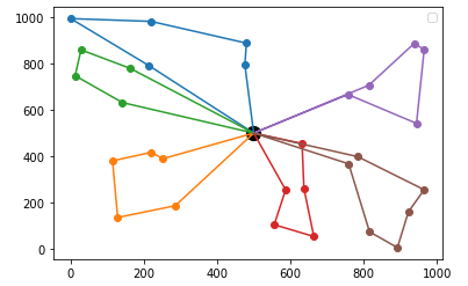
\includegraphics[width=0.5\textwidth]{Gambar/Picture1.png}
  \caption{Contoh MTSP 6 klaster}
  \label{fig:mtsp6}
\end{figure}

\begin{figure}[H]
  \centering
  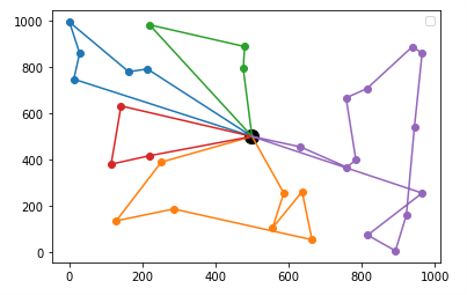
\includegraphics[width=0.5\textwidth]{Gambar/Picture2.png}
  \caption{Contoh MTSP 5 klaster}
  \label{fig:mtsp5}
\end{figure}

\subsection{Algoritma}

Maulana menyebutkan dalam artikelnya algoritma adalah kumpulan perintah untuk menyelesaikan suatu masalah dan diselesaikan dengan cara sistematis, terstruktur dan logis \cite{maulana2017pembelajaran}. Algoritma digunakan untuk memcahkan permasalahan yang dialami oleh seorang pengguna program.

\subsection{Algoritma $k$-means}

$K$-Means adalah jenis metode klasifikasi tanpa pengawasan yang mempartisi item data menjadi satu atau lebih klaster \cite{agusta2007k}. $K$-Means mencoba untuk memodelkan suatu dataset ke dalam beberapa klaster sehingga item-item data dalam suatu klaster memiliki karakteristik yang sama dan memiliki karakteristik yang berbeda dengan klaster lainnya.

Menurut S Monalisa \cite{monalisa2018klasterisasi} tahapan mengklaster menggunakan algoritma \textit{k}-means adalah sebagai berikut.

\begin{enumerate}
	\item Menentukan banyak klaster
	\item Memilih beberapa \textit{centroid} secara acak sesuai banyak klaster
	\item Hitung jarak titik ke centroid dengan rumus \textit{Euclidean distance} seperti Persamaan (\ref{eq:euclidean1}).
	\begin{equation}
	d_{xy}=\sqrt{\sum_{i=1}^{n}(x_i-y_i)^{2}}
	\label{eq:euclidean1}
	\end{equation}
	\item Titik-titik yang tersebar masuk ke klaster yang sama dengan titik \textit{centroid} yang paling dekat
	\item Perbarui \textit{centroid} dengan menghitung nilai rata-rata nilai pada masing-masing klaster
	\item Lakukan iterasi sebanyak mungkin dengan kembali ke tahapan 3 sampai tidak ada perubahan klaster atau perubahan nilai \textit{centroid}
\end{enumerate}

\subsection{Centroid}

Centroid adalah nilai yang dijadikan sebagai titik awal dimulainya sebuah pengelompokan (\textit{clustering}) pada algoritma $k$-means \cite{retno2019peningkatan}. Untuk melakukan pengelompokan data, dimulai dengan menghitung jarak dari setiap titik tujuan menuju ke setiap titik centroid sebagai awal pembentukan klaster, setelah itu titik-titik tujuan akan dikelompokkan menurut titik klaster terdekatnya. Dalam langkah tersebut akan dihitung titik-titik centroid yang baru menggunakan nilai rata-rata titik dari tiap klaster.

\subsection{Algoritma Genetika}

Pada artikel Hermanto disebutkan bahwa algoritma genetika adalah algoritma yang digunakan untuk mencari solusi suatu permasalahan dengan cara yang lebih alami yang terispirasi dari teori evolusi  \cite{hermawanto2003algoritma}. Dalam hal ini, algoritma genetika dapat juga digunakan untuk pencarian sebuah rute terpendek dalam sebuah kasus perjalanan.

Menurut Armanda RS \cite{armanda2016penerapan} dalam artikelnya menyampaikan penyelesaian masalah menggunakan algoritma genetika memerlukan beberapa tahapan sebagai berikut:

\begin{enumerate}
	\item Menyiapkan populasi, dalam penelitian ini yang digunakan adalah data yang telah diklaster menggunakan algoritma \textit{k}-means
	\item Melakukan reproduksi dengan \textit{crossover} dan mutasi pada pembentukan awal populasi
	\item Seleksi dengan metode elitism
	\item Menentukan nilai fitness agar mendapatkan solusi akhir yang optimal
	\item Iterasi dilakukan untuk generasi berikutnya.
\end{enumerate}

\subsection{Fitness}
Fitness adalah suatu ukuran yang dijadikan acuan untuk mengetahui baik atau tidaknya suatu individu atau bisa disebut nilai dari fungsi tujuan \cite{basuki2003strategi}. Tujuan dari penggunaan algoritma genetika adalah untuk mengoptimalkan nilai fitness dengan cara mencari nilai fitness yang paling maksimal atau minimal. Seperti dalam penelitian ini yang tujuannya adalah mencari jarak yang paling minimal maka nilai fitness nya yang dicari adalah yang paling minimal juga.

\subsection{\textit{Crossover}}
\textit{Crossover} atau persilangan adalah operator dari algoritma genetika yang melibatkan dua induk untuk membentuk kromosom baru menurut artikel \cite{hardi2014analisis}. Dalam langkah ini dilakukan dengan cara menukar sebagian gen pada kromosom induk pertama dengan gen pada kromosom induk kedua seperti pada Gambar \ref{fig:crossover}. Proses \textit{crossover} tersebut diterapkan pada setiap individu dengan probabilitas \textit{crossover} ($p_c$) yang telah ditentukan. Jika diterapkan \textit{crossover} keturunan didapatkan dari kromosom-kromosom induk. Namun jika \textit{crossover} tidak diterapkan satu induk dipilih secara acak dengan $p_c$ yang sama dan diduplikasi menjadi anak.

\begin{figure}[H]
  \centering
  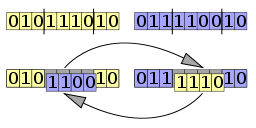
\includegraphics[width=0.5\textwidth]{Gambar/crossover.png}
  \caption{Proses crossover}
  \label{fig:crossover}
\end{figure}

\subsection{Mutasi}
Mutasi atau mutation adalah operator yang digunakan untuk mengubah gen-gen yang terdapat dalam kromosom. Model dalam proses ini sebagaimana yang terjadi dalam kehidupan alam \cite{rovie2014genetic} seperti pada Gambar \ref{fig:mutasi}. Dalam proses mutasi akan dibangkitkan sebuah bilangan acak sebagai Probabilitas mutasi ($p_m$) yang sangat kecil. Mutasi diterapkan dengan tujuan untuk memperoleh nilai fitness yang lebih baik dari sebelumnya, dan lama-kelamaan akan menjadi solusi optimum yang diinginkan.

\begin{figure}[H]
  \centering
  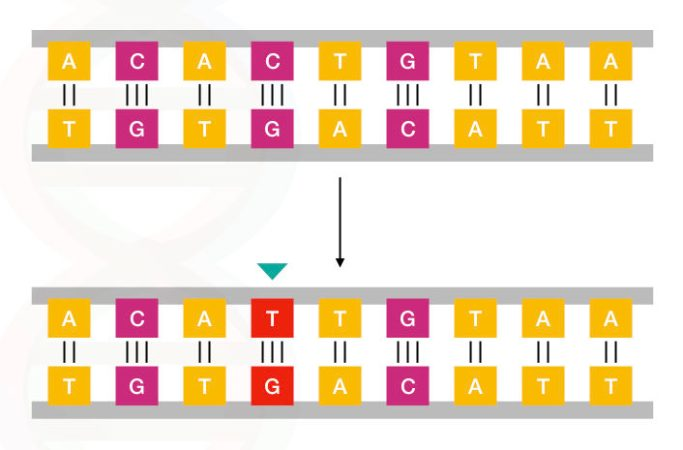
\includegraphics[width=0.5\textwidth]{Gambar/mutasi.jpg}
  \caption{Proses mutasi}
  \label{fig:mutasi}
\end{figure}